 % !TeX document-id = {f19fb972-db1f-447e-9d78-531139c30778}
% !BIB program = biber

%\documentclass[handout]{beamer}
\documentclass[compress]{beamer}
\usepackage[T1]{fontenc}
\usetheme[block=fill,subsectionpage=progressbar,sectionpage=progressbar]{metropolis} 
\usepackage{graphicx}

\usepackage{wasysym}
\usepackage{etoolbox}
\usepackage[utf8]{inputenc}

\usepackage{threeparttable}
\usepackage{subcaption}

\usepackage{tikz-qtree}
\setbeamercovered{still covered={\opaqueness<1->{5}},again covered={\opaqueness<1->{100}}}


% color-coded listings; replace those above 
\usepackage{xcolor}
\usepackage{minted}
\definecolor{listingbg}{rgb}{0.87,0.93,1}
\setminted[python]{
	frame=none,
	framesep=1mm,
	baselinestretch=1,
	bgcolor=listingbg,
	fontsize=\scriptsize,
	linenos,
	breaklines
}



\usepackage{listings}

\lstset{
	basicstyle=\scriptsize\ttfamily,
	columns=flexible,
	breaklines=true,
	numbers=left,
	%stepsize=1,
	numberstyle=\tiny,
	backgroundcolor=\color[rgb]{0.85,0.90,1}
}


\lstnewenvironment{lstlistingoutput}{\lstset{basicstyle=\footnotesize\ttfamily,
		columns=flexible,
		breaklines=true,
		numbers=left,
		%stepsize=1,
		numberstyle=\tiny,
		backgroundcolor=\color[rgb]{.7,.7,.7}}}{}


\lstnewenvironment{lstlistingoutputtiny}{\lstset{basicstyle=\tiny\ttfamily,
		columns=flexible,
		breaklines=true,
		numbers=left,
		%stepsize=1,
		numberstyle=\tiny,
		backgroundcolor=\color[rgb]{.7,.7,.7}}}{}



\usepackage[american]{babel}
\usepackage{csquotes}
\usepackage[style=apa, backend = biber]{biblatex}
\DeclareLanguageMapping{american}{american-UoN}
\addbibresource{../../literature.bib}
\renewcommand*{\bibfont}{\tiny}

\usepackage{tikz}
\usetikzlibrary{shapes,arrows,matrix}
\usepackage{multicol}

\usepackage{subcaption}

\usepackage{booktabs}
\usepackage{graphicx}



\makeatletter
\setbeamertemplate{headline}{%
	\begin{beamercolorbox}[colsep=1.5pt]{upper separation line head}
	\end{beamercolorbox}
	\begin{beamercolorbox}{section in head/foot}
		\vskip2pt\insertnavigation{\paperwidth}\vskip2pt
	\end{beamercolorbox}%
	\begin{beamercolorbox}[colsep=1.5pt]{lower separation line head}
	\end{beamercolorbox}
}
\makeatother



\setbeamercolor{section in head/foot}{fg=normal text.bg, bg=structure.fg}



\newcommand{\question}[1]{
	\begin{frame}[plain]
		\begin{columns}
			\column{.3\textwidth}
			\makebox[\columnwidth]{
				
\includegraphics[width=\columnwidth,height=\paperheight,keepaspectratio]{../../pictures/mannetje.png}}
			\column{.7\textwidth}
			\large
			\textcolor{orange}{\textbf{\emph{#1}}}
		\end{columns}
\end{frame}}



\title[Teach-the-teacher: Python]{\textbf{Teach-the-teacher: Python} 
\\Day 4: »Processing textual data // NLP« }
\author[Anne Kroon]{Anne Kroon\\ \footnotesize{a.c.kroon@uva.nl}}
\date{December 4, 2023}
\institute[UvA CW]{UvA RM Communication Science}


\begin{document}
	
	\begin{frame}{}
		\titlepage{\tiny }
	\end{frame}
	
	\begin{frame}{Today}
		\tableofcontents
	\end{frame}


\section{Bottom-up vs. top-down}

\begin{frame}[standout]
Automated content analysis can be either \textcolor{red}{bottom-up} (inductive, explorative, pattern recognition, \ldots) or \textcolor{red}{top-down} (deductive, based on a-priori developed rules, \ldots). Or in between.
\end{frame}


\begin{frame}{The ACA toolbox}
\makebox[\columnwidth]{
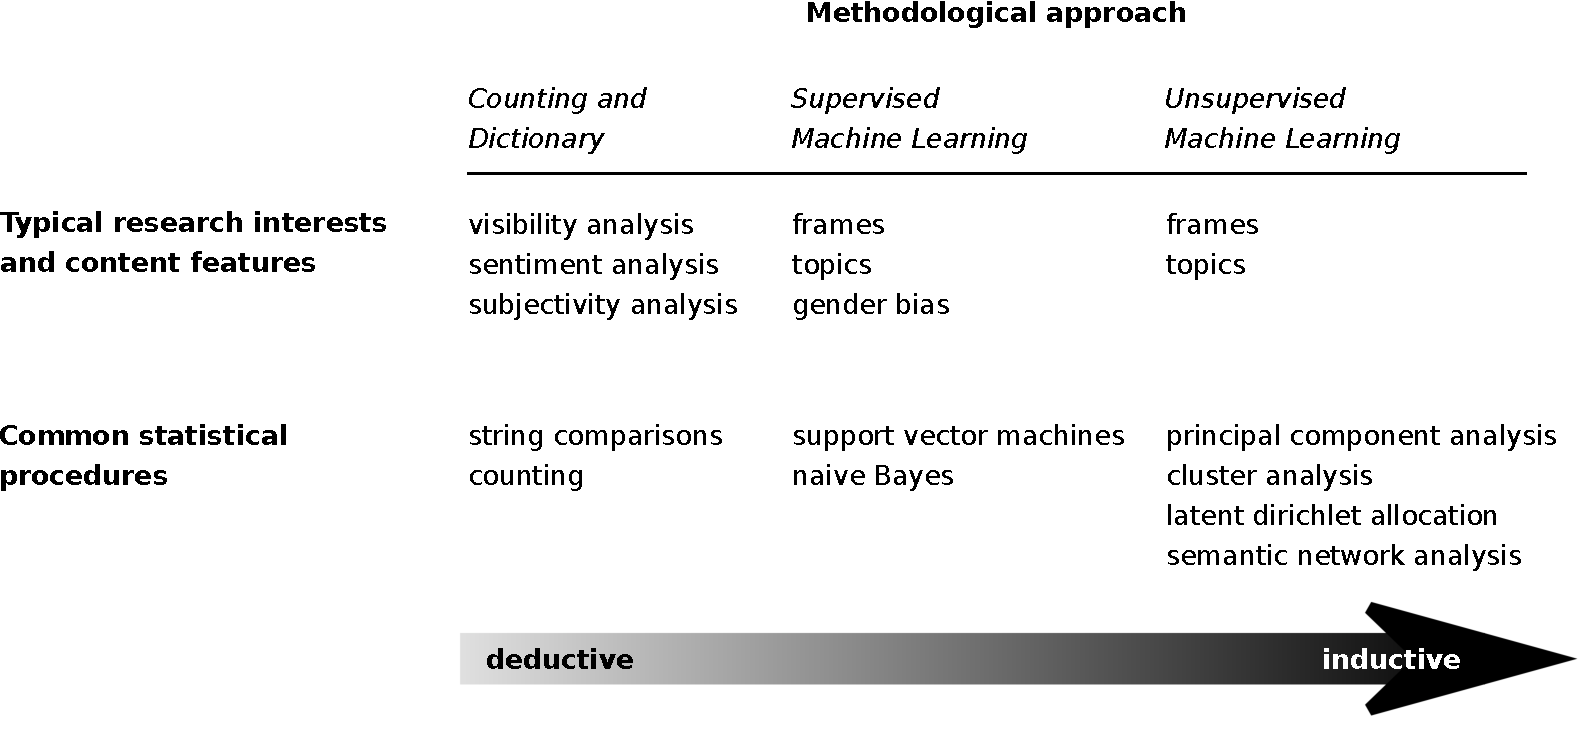
\includegraphics[width=\columnwidth,height=\paperheight,keepaspectratio]{../../media/boumanstrilling2016}}
\\
\cite{Boumans2016}
\end{frame}


\begin{frame}{Bottom-up vs. top-down}
\begin{block}{Bottom-up}
\begin{itemize}
\item Count most frequently occurring words 
\item Maybe better: Count combinations of words $\Rightarrow$ Which words co-occur together?
\end{itemize}
We \emph{don't} specify what to look for in advance	
\end{block}

\onslide<2>{
\begin{block}{Top-down}
\begin{itemize}
	\item Count frequencies of pre-defined words
	\item Maybe better: patterns instead of words
\end{itemize}
We \emph{do} specify what to look for in advance	
\end{block}
}
\end{frame}


\begin{frame}[fragile]{A simple bottom-up approach}
\begin{lstlisting}
from collections import Counter

texts = ["I really really really love him, I do", "I hate him"]

for t in texts:
    print(Counter(t.split()).most_common(3))
\end{lstlisting}
\begin{lstlistingoutput}
[('really', 3), ('I', 2), ('love', 1)]
[('I', 1), ('hate', 1), ('him', 1)]
\end{lstlistingoutput}
\end{frame}


\begin{frame}[fragile]{A simple top-down approach}
\begin{lstlisting}
texts = ["I really really really love him, I do", "I hate him"]
features = ['really', 'love', 'hate']

for t in texts:
    print(f"\nAnalyzing '{t}':")
    for f in features:
        print(f"{f} occurs {t.count(f)} times")
\end{lstlisting}
\begin{lstlistingoutput}
Analyzing 'I really really really love him, I do':
really occurs 3 times
love occurs 1 times
hate occurs 0 times

Analyzing 'I hate him':
really occurs 0 times
love occurs 0 times
hate occurs 1 times

\end{lstlistingoutput}
\end{frame}

\question{When would you use which approach?}


\begin{frame}{Some considerations}
\begin{itemize}[<+->]
	\item Both can have a place in your workflow (e.g., bottom-up as first exploratory step)
	\item You have a clear theoretical expectation? Bottom-up makes little sense.
	\item But in any case: you need to transform your text into something ``countable''.
\end{itemize}
\end{frame}


\input{../../modules/working-with-text/basic-string-operations.tex}
\input{../../modules/working-with-text/bow.tex}

\begin{frame}[fragile]{General approach}
\Large

\textcolor{red}{Test on a single string, then make a for loop or list comprehension!}

\pause

\normalsize

\begin{alertblock}{Own functions}
If it gets more complex, you can write your ow= function and then use it in the list comprehension:
\begin{lstlisting}
def mycleanup(t):
    # do sth with string t here, create new string t2
    return t2

results = [mycleanup(t) for t in allmytexts]
\end{lstlisting}
\end{alertblock}
\end{frame}


\begin{frame}[fragile]{Pandas string methods as alternative}
If you select column with strings from a pandas dataframe, pandas offers a collection of string methods (via \texttt{.str.}) that largely mirror standard Python string methods:

\begin{lstlisting}
df['newcoloumnwithresults'] = df['columnwithtext'].str.count("bla")
\end{lstlisting} 


\pause

\begin{alertblock}{To pandas or not to pandas for text?}
Partly a matter of taste. 

Not-too-large dataset with a lot of extra columns? Advanced statistical analysis planned? Sounds like pandas.

It's mainly a lot of text? Wanna do some machine learning later on anyway? It's large and (potentially) messy? Doesn't sound like pandas is a good idea.
\end{alertblock}

\end{frame}



%\begin{frame}[plain]
%	\printbibliography
%\end{frame}



\end{document}



